\section{Evaluation}
\label{sec:eval}

We evaluate our cuckoo hash by directly comparing it's
performance in terms of latency and throughput with other
state of the art disaggregated key value stores. We
substantiate our design decisions through a series of
micro-benchmarks. We measure throughput as a response to
hashing factor, read threshold, and search algorithm.

\begin{figure*}[ht]
    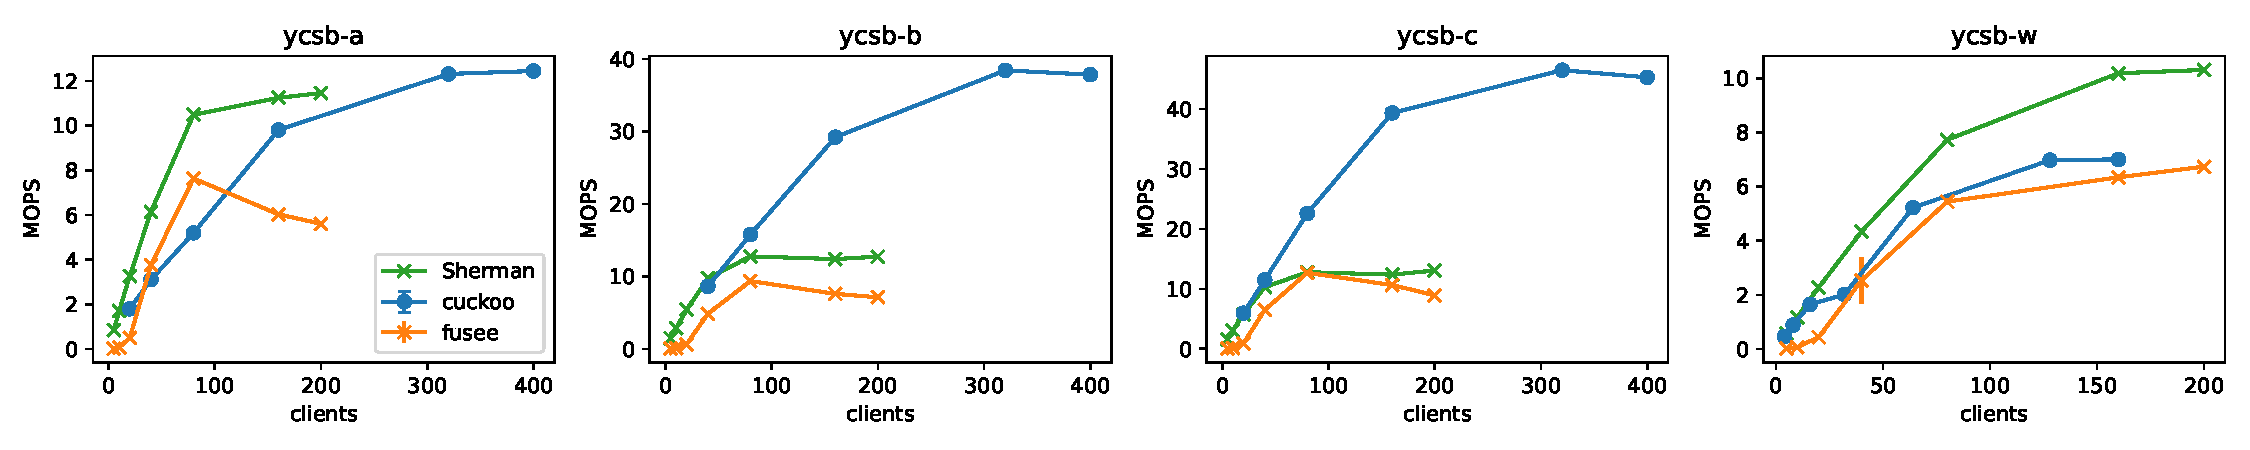
\includegraphics[width=0.99\linewidth]{fig/hero_ycsb_throughput.pdf}
    \caption{race vs rcuckoo simulated throughput \todo{rerun ycsb-b numbers don't look quite right}}
    \label{fig:ycsb_throughput}
\end{figure*}

\begin{figure*}[ht]
    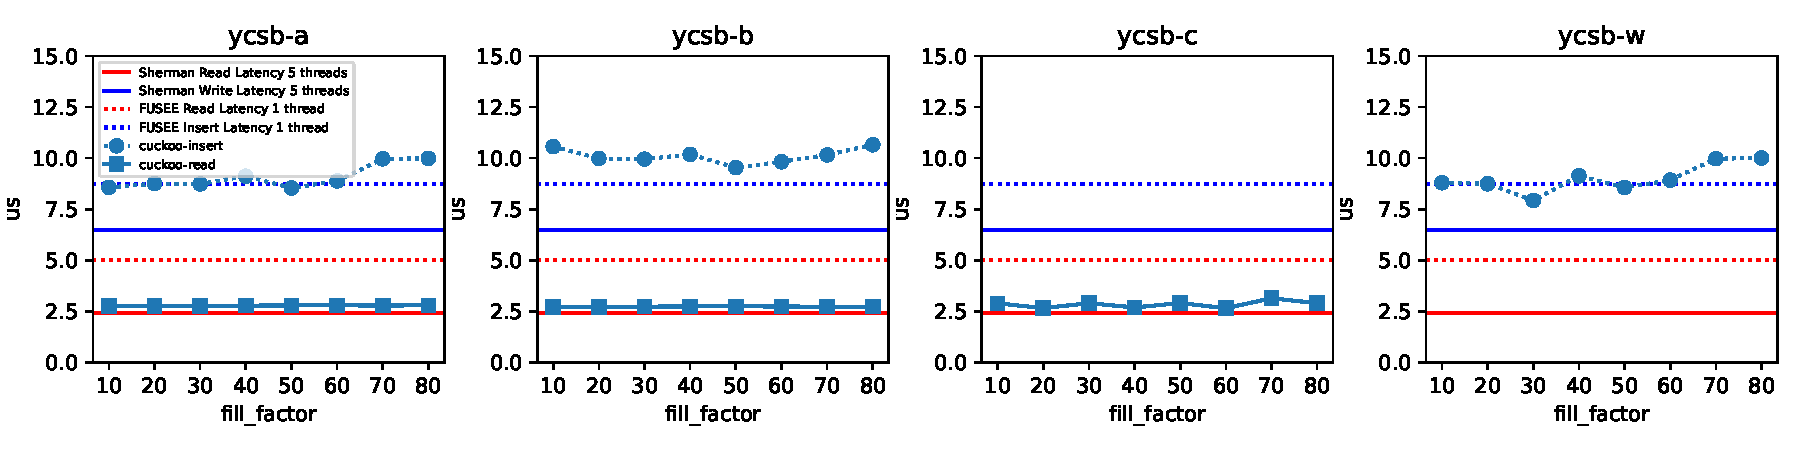
\includegraphics[width=0.99\linewidth]{fig/hero_ycsb_fill_latency.pdf}
    \caption{race vs rcuckoo workload fill latency}
    \label{fig:ycsb_fill_latency}
\end{figure*}

\begin{figure}[ht]
    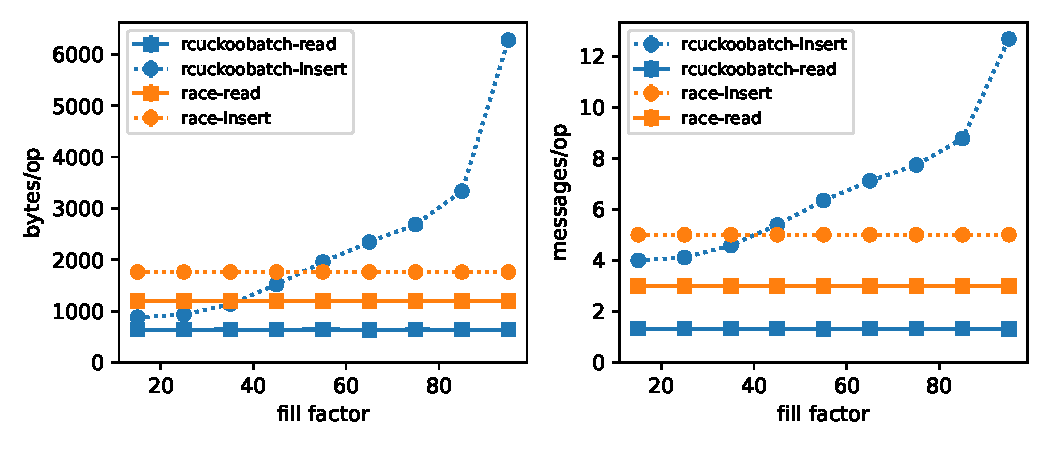
\includegraphics[width=0.99\linewidth]{fig/hero_ycsb_fill_ops_bw.pdf}
    \caption{YCSB-A workload messages and bandwidth per operation as a function of fill factor}
    \label{fig:ycsb_fill_ops_bw}
\end{figure}

\begin{figure}[ht]
    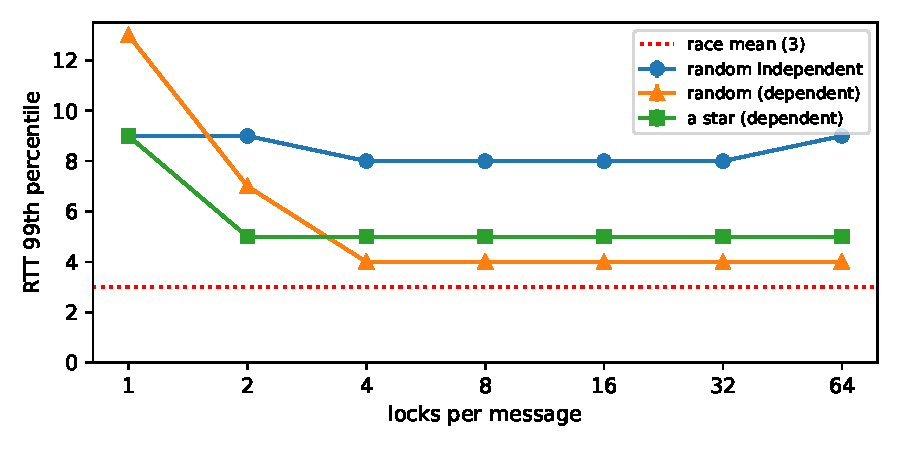
\includegraphics[width=0.99\linewidth]{fig/search_dependence.pdf}

    \caption{Round trips per insert operation compared
    across search functions and hash functions. Dependent
    hash functions with A* have the shortest search
    times.~\todo{latest numbers for A* are counter intuitive
    - dig into}}

    \label{fig:search_dependence}
\end{figure}

\subsection{Setup}

Our evaluate setup is an 11 node cluster of dual socket
Intel machines. Each CPU is an Intel Xeon(R) E5-2650 clocked
at 2.20GHz. Each machine has 256GB of RAM with 128GB per
NUMA node. All machines have a single dual socket ConnectX-5
attached to a 100GBPs Mellanox Onyx switch. In our
experiments for RCuckoo we use one sever as a memory server,
and the rest a client machines spreading out client threads
evenly across machines.

\subsection{Systems}

\subsubsection{FUSEE}

FUSEE is a remote memory key-value store designed for full
disaggregation~\cite{fusee}.  It is built on top of
RACE~\cite{race} with extensions to support replication in
the face of contention.  Currently RCuckoo does not support
replication, our FUSEE setup uses a single memory node to
effectively remove the overhead of replication. RACE is the
most similar system in terms of assumptions to RCuckoo,
however no open source implementation of RACE is available.
RACE hashing uses fixed sized 64 bit index entries to
support RDMA compare and swap operation width. As such RACE
based systems cannot store key value pairs in the index and
must use a second round trip on reads to recover extent
entries which contain full key value pairs.

\subsubsection{Sherman}

Sherman is a remote memory b-tree designed for write
optimization. Sherman clusters are not fully disaggregated.
Each node in a sherman cluster has many CPU cores, and a
single memory core. The memory core is responsible for
servicing allocation RPC calls from clients. Sherman is
similar to RCuckoo in that it uses locks to guard access.
However, it assumes that colocated clients can resolve lock
contention locally. These assumptions enable sherman to have
high performance under contention, and enable fast reads as
the B-tree leaf nodes can be right sized by the memory
allocator. While Sherman does not meet the fully
disaggregated model it does provide a good comparison for
RCuckoo as it is the only other system to use locks in
remote memory.


\subsubsection{Clover}
\todo{insert a short clover description}

\subsection{System Performance}

\textbf{Throughput:} Figure~\ref{fig:ycsb_throughput} shows
the throughput of FUSEE, Sherman and RCuckoo for YCSB
workloads. YCSB-W is a 100\% write workload. YCSB-A is a
50\% read 50\% write workload. YCSB-B is 95\% read and 5\%
write, and YCSB-C is 100\% read.  In each experiment clients
fill the hash table from empty to 50\% full on tables with
10M 32bit keys and 32bit values. For read only workloads the
hash table is first filled to 50\% and then clients read
from the table.  

Rcuckoo is competitive on insert heavy workloads and is able
to slightly outperform FUSEE on write only workloads.
RCuckoo shines on read heavy workloads as each read requires
only a single rounds trip, and approximately 60\% of reads
only require a single RDMA packet. On each of these
benchmarks our read threshold is set to a max of 256 bytes.
On read only workloads RCuckoo is able to outperform FUSEE
and Sherman by 2x ~\todo{double check sherman, I feel like
it should be able to get a better value for read only..}


\textbf{Latency:} 

RCuckoo Latency is shown across each YCSB workload in
Figure~\ref{fig:ycsb_fill_latency}. In each of these
experiments we fill the table to a given fill factor, and
then run the workload for 100k operations. In each case
RCuckoo holds a near constant latency. These experiments are
run at low contention to illustrate only the response to
fill factor not contention. Independent measurements from
Sherman and FUSEE show their minimum latencies for
individual operations (not taken as part of the workload) to
illustrate their relative performance.

%%
% Figure~\ref{fig:ycsb_fill_latency}, shows the average
% operation latency for each workload. Here average RTT is the
% average between both reads and writes. RACE incurs
% additional round trips from reading from its extent and
% from verifying its successful inserts. RACE has very few
% collisions as its critical section for insertion is the
% duration of a single RDMA CAS. Few of RACE's inserts fail
% and it retains near constant latency for read and writes
% across all fill factors. The same is true for rcuckoo reads
% which remain at a single round trip. Rcuckoo inserts are
% subject to additional round trips as the table fills.  Most
% additional round trips are caused by locks being spaced
% further than the span of an RDMA CAS on the lock table. Some
% are caused by contention. The small improvement of ycsb-a
% and ycsb-b over ycsb-w inserts are due to reduced write
% contention from the workload.

\textbf{Bandwidth, and messages:} 
\todo{todo}
% Rcuckoo design trades off
% bandwidth for latency by increases the size of reads for all
% operations. We measure the effect of fill factor on the
% bandwidth and messages required per operation with the same
% experiment used to measure latency.
% Figure~\ref{fig:ycsb_fill_ops_bw} shows how rcuckoo and
% RACE's messages and bandwidth respond to fill factor. At low
% fill rates (less than 50\%) rcuckoo uses less bandwidth per
% operation and less messages per operation than RACE. Above
% 50\% collisions in the hash table increase the cost of
% insertions. While the size of the cuckoo path does not
% directly relate to the number of round trips, it does
% directly relate to messages. High fill factors nearly double
% the number of insert messages required to perform insertions
% with rcuckoo, and bandwidth can increase by up to a factor of
% 4. \todo{In the future we could perform very large writes to
% reduce the number of messages at the cost of more
% bandwidth.}

\textbf{Locks per message and independence:}
\todo{run this experiment with many machines}

% Hash function
% locality hash a major impact in rcuckoo's performance.
% Acquiring locks can only be done in a few round trips when
% the locks are clustered together tightly in the lock table.
% Furthermore, the search function used to determine the
% cuckoo path has a large impact on the locality of the locks
% necessary to lock the path. We evaluate dependent hashing
% and independent hashing as well as random and a* search. We
% measure the number of round trips required for each control
% as a function of the number of locks which can be acquired
% per round trip.

% Figure~\ref{fig:search_dependence} shows the performance
% improvements gained by both locality hashing and A* search.
% In this experiment the table is filled from 0 to 90\% full
% with a ycsb-w workload. We measure the 99th percentile of
% round trips for these workloads. Random search with
% independent hashing leads to a large number of round trips
% as locks are scattered throughout the table. RDMA masked CAS
% operation do little here to reduce the round trips as they
% can rarely aquire more than one lock in a round trip. With
% dependent hashing and random search RDMA CAS operation are
% almost sufficient to reduce round trips, however the absolute
% number of locks required per insert is high which leads to
% greater contention. A* search with dependent hashing has
% cuckoo paths that are both short, and clustered together.



\subsection{Search Performance:}

\todo{\textbf{A* search vs BFS:} We compare the performance of A*
vs BFS for locally computed insertions. A* performance
directly effects system throughput as this algorithm is run
twice on every insert.}

\todo{\textbf{Hashing Algoritms:} Rcuckoo hashing requires
executing many hash compuations. We evaluate our A* search
alorithm abolute performacne on various hash functions and
show how this values effect our overall fill factors.}

\begin{figure*}[t]
    \centering
    \begin{subfigure}{0.3\linewidth}
        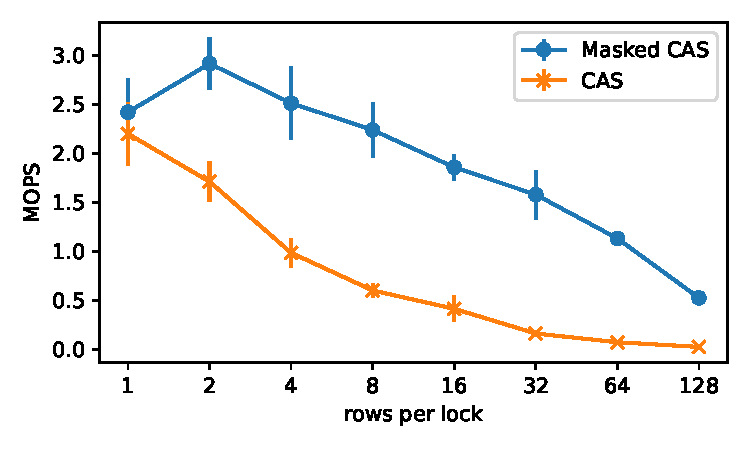
\includegraphics[width=0.99\linewidth]{fig/masked_cas_lock_size.pdf}
    \end{subfigure}
    \begin{subfigure}{0.3\linewidth}
        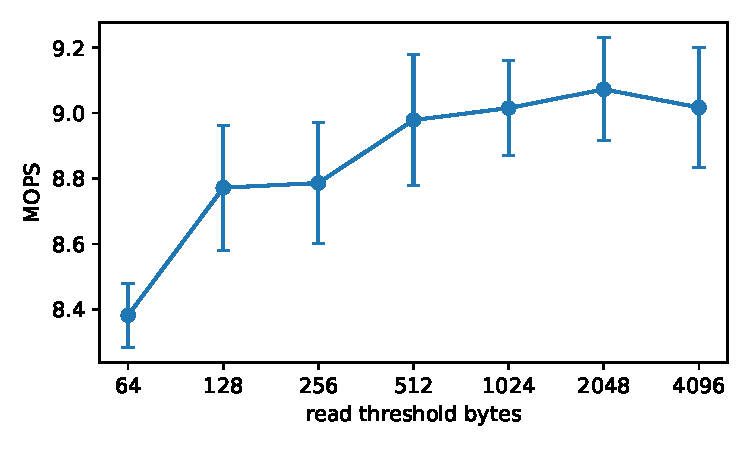
\includegraphics[width=0.99\linewidth]{fig/read_size.pdf}
        % \label{fig:hash_factor}
        % \caption{}
    \end{subfigure}
    \begin{subfigure}{0.3\linewidth}
        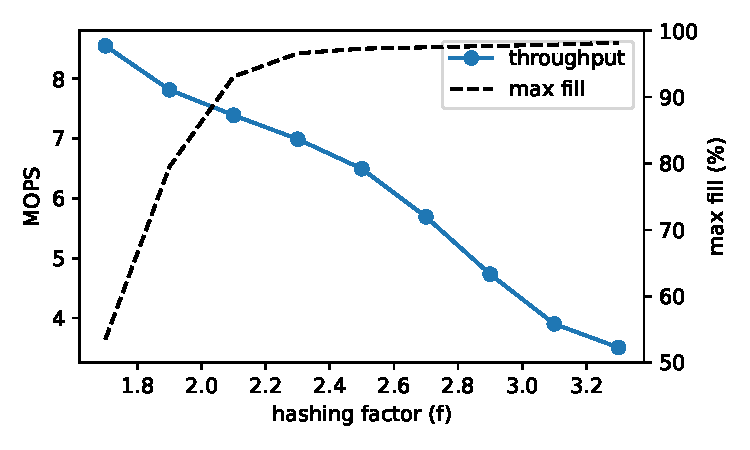
\includegraphics[width=0.99\linewidth]{fig/factor.pdf}
        % \label{fig:hash_fill}
        % \caption{}
    \end{subfigure}.
    \vspace{-1em}
    \caption{
    \textbf{(a)} Masked CAS vs Unmasked CAS throughput.
    \textbf{(b)} Read threshold vs throughput.
    \textbf{(c)} Exponential factor relation to max fill in cuckoo hash.
    }
    \label{fig:performance_breakdown}

\end{figure*}

\subsubsection{Masked CAS}

Under contention masked CAS operations provide a significant
performance improvement. We measure their benefit in terms
of throughput by comparing them with default CAS. In the
default case, when acquiring locks clients set the lock bits
for the locks they require and set all other bits in the cas
to 0. If the cas fails the current state of the lock table
over that range is returned as a result to the client and
the client tries to aquire their locks again using the
updated state of the lock table. Masked compare and swaps
are issued with the minimal mask required to set the locks.

We measure the performance improvement at high fill rates
(85-90\%) on write only workloads and vary the number of
rows per lock on each experiment.
Figure~\ref{fig:performance_breakdown} shows the improvement
gained by masked CAS. Default CAS operations perform better
with fewer rows per lock, as the probability of a lock being
set within the 64bit range is at its lowest. At higher rows
per lock CAS suffers from failed lock acquisitions from both
contested locks and due to a lack of synchronization. In
contrast masked CAS sees an improvement when two rows per
lock are used, as more second search attempts succeed, and
only suffers from direct lock contention as the rows per
lock increase.


\subsection{Hash Function Factor $f$}

\todo{we vary f to show the tradeoff between maximum fill factor and throughput}

\subsection{Read Threshold Performance}



As described in section ~\ref{sec:reading} rcuckoo uses a
read threshold to capture both hash locations if the
locations are within a defined read threshold.
Figure~\ref{fig:read_threshold} shows the performance gains
from increasing the read threshold. Here each row is 64
bytes so our minimum threshold of 64 ensures two packets are
issued for each read request. Higher read thresholds trade
off network bandwidth for operation latency. When bandwidth
is plentiful large windows can improve throughput but up to
8\%.

% \begin{figure}[ht]
%     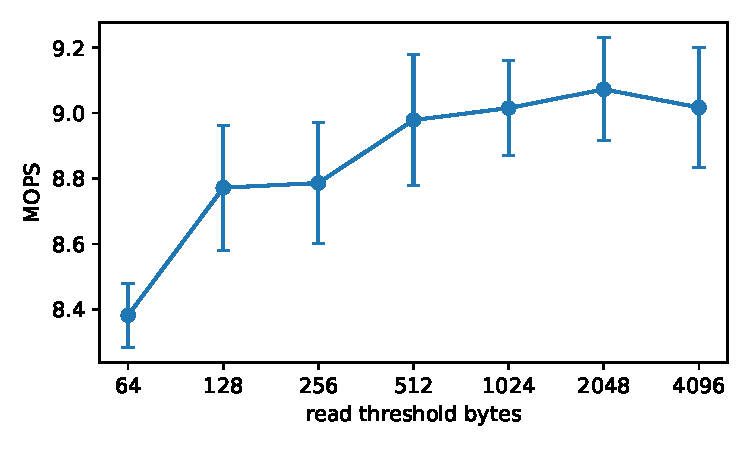
\includegraphics[width=0.99\linewidth]{fig/read_size.pdf}
%     \caption{Read Threshold vs Throughput}
%     \label{fig:read_threshold}
% \end{figure}


\subsection{Entry Size}

Key value pairs embedded directly in the index enable single
round trip reads, at the cost of inflating write bandwidth.
Large row sizes increase the size of reads during locking
and search. Figure~\cite{fig:entry_size} shows the effect of
key value pair size on operation throughput. YCSB-A
workloads saturate network bandwidth and thus decrease in
throughput as a function of entry size. In contrast YCSB-C
is largely unaffected by entry size. \sg{We suggest that
pairs larger than 64 bytes use extents rather than embedding
directly in the index.}


\begin{figure}[ht]
    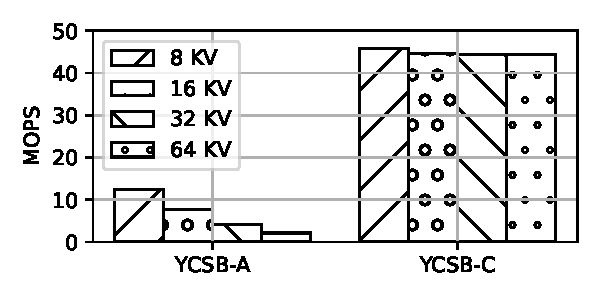
\includegraphics[width=0.99\linewidth]{fig/entry_size.pdf}
    \caption{Throughput vs KV entry size}
    \label{fig:entry_size}
\end{figure}

